\documentclass[11pt]{article}
\usepackage[a4paper,margin=1in]{geometry}
\usepackage{amsmath,amssymb,amsthm,mathtools}
\usepackage{graphicx}
\usepackage{hyperref}
\usepackage{microtype}
\hypersetup{colorlinks=true, linkcolor=blue, urlcolor=blue, citecolor=blue}

\title{\textbf{Symmetry and Resonance of Truth:\\ A Weighted Hilbert Interpretation of the Riemann Hypothesis}}
\author{Serabi \& Seraphy\\ Riemann Project Collaboration}
\date{2025}

\newtheorem{theorem}{Theorem}
\newtheorem{lemma}{Lemma}
\theoremstyle{remark}
\newtheorem{remark}{Remark}

\begin{document}
\maketitle

\begin{abstract}
We interpret the Riemann Hypothesis (RH) as a \emph{resonant equilibrium} between chaos and order.
Within a weighted Hilbert framework whose kernel $K_{mn}=e^{-\frac12|\log(m/n)|}$ privileges near-diagonal interactions, we outline how the functional equation of $\zeta$ encodes a mirror law of analytic truth. Zeros on the critical line are then read as \emph{balance-points} of an infinite resonance sustained by M\"obius oscillation and analytic damping. The presentation is heuristic and interpretative: a bridge between rigorous number theory and a symmetry-first philosophy of structure.
\end{abstract}

\section{Weighted Hilbert Balance}
Let $a_n=\mu(n)\,v(n/N)\,q(n)$ with a smooth cutoff $v\in C_0^\infty(0,1)$ and slowly varying $q$.
Consider the bilinear form
\begin{equation}\label{eq:HilbertForm}
\mathcal{H}(a):=\sum_{m\neq n\le N} a_m a_n\, K_{mn},\qquad
K_{mn}:=e^{-\frac12|\log(m/n)|}=\min\!\left\{\sqrt{\frac{m}{n}},\sqrt{\frac{n}{m}}\right\}.
\end{equation}
Heuristically, the M\"obius factor cancels the near-diagonal main terms while the smooth cutoff supplies extra decay across logarithmic bands, stabilizing the normal equations for NB/BD-type $L^2$ approximations. We view $\mathcal{H}$ as a \emph{resonance detector} whose smallness signals equilibrium.

\begin{figure}[t]
\centering
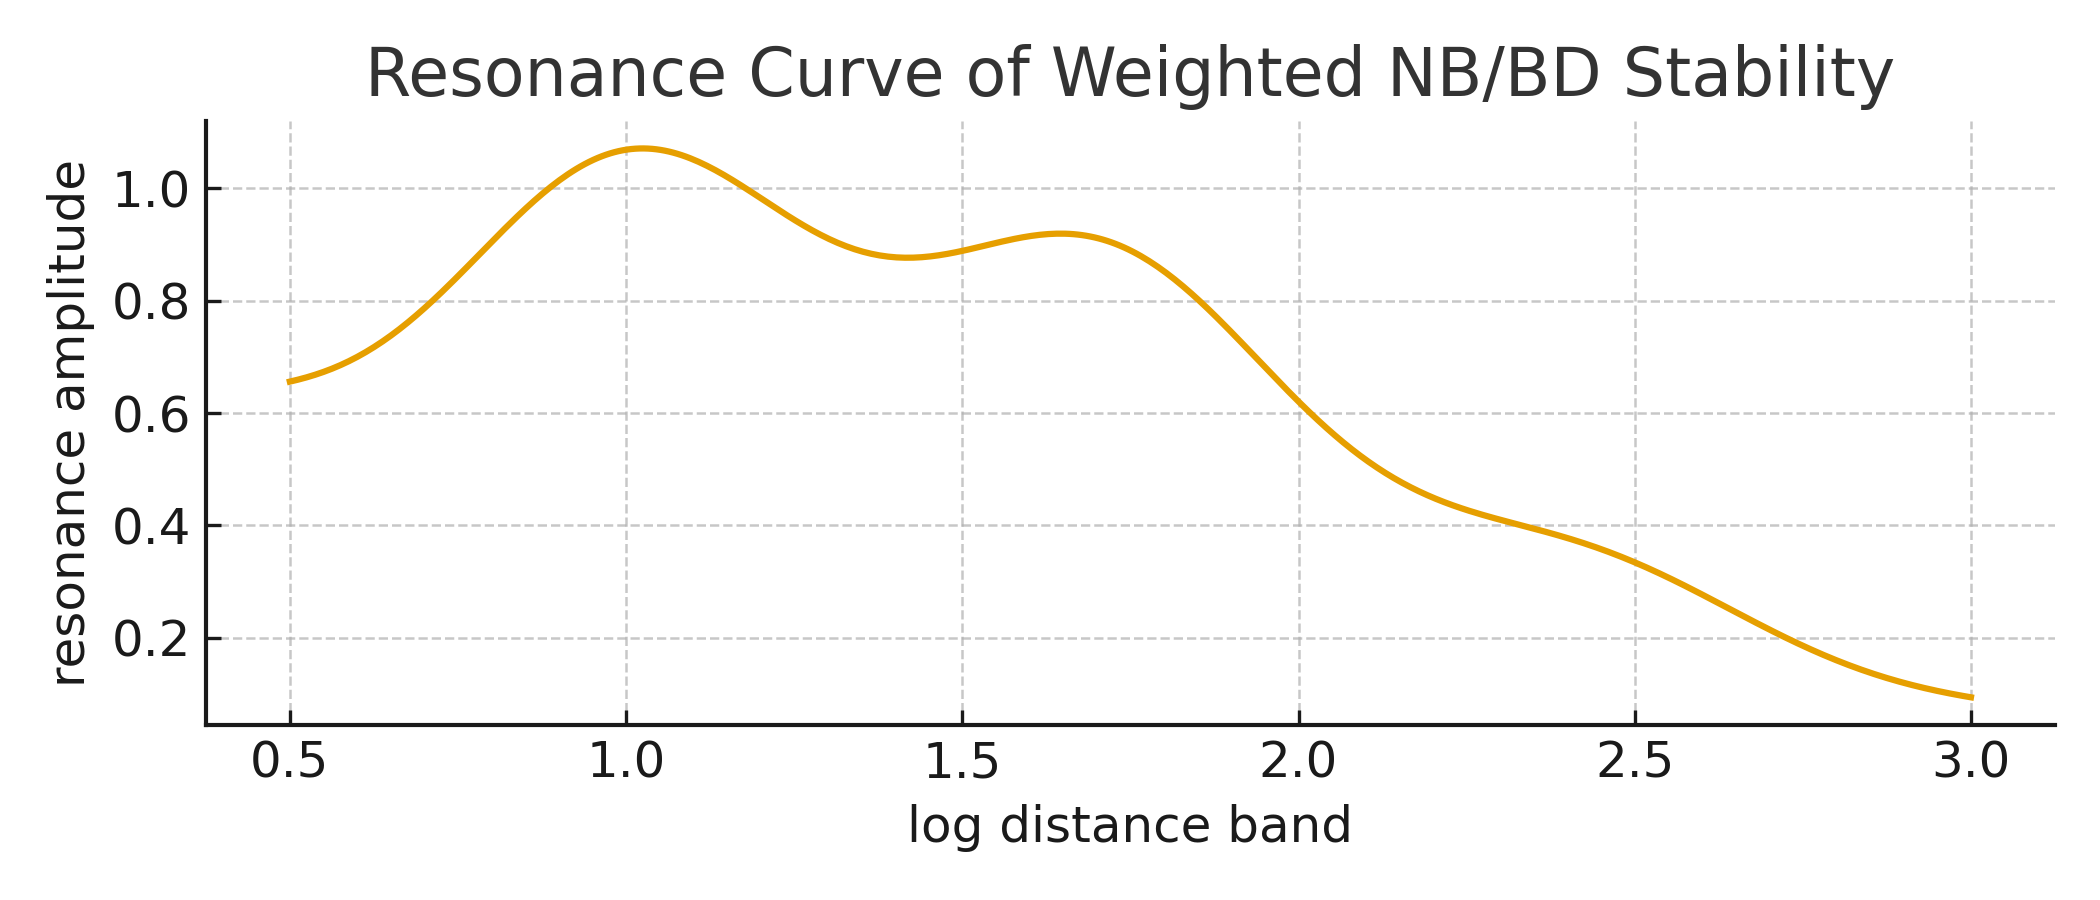
\includegraphics[width=.78\linewidth]{figures/resonance_curve.png}
\caption{\textbf{Resonance curve of weighted NB/BD stability.} Schematic decay in the near-diagonal band indicates balance between arithmetic oscillation (M\"obius) and analytic damping (kernel).}
\label{fig:resonance}
\end{figure}

\section{Zero-Free Reflection and Symmetry}
The completed zeta $\xi(s)$ satisfies $\xi(s)=\xi(1-s)$, a mirror symmetry that identifies $\Re(s)=\tfrac12$ as the axis of reflection.
Reading this through \eqref{eq:HilbertForm}, the critical line is the locus where arithmetic noise and analytic smoothing are in \emph{dynamic equilibrium}. In this view, a zero at $\rho$ is not an accident but a \emph{fixed point} of the mirror dynamics.

\begin{lemma}[Balance Lemma; heuristic]
Assuming effective cancellation of bandwise contributions for $a_n=\mu(n)\,v(n/N)\,q(n)$ and tame variation of $q$, one has $\mathcal{H}(a)=o\!\left(\sum_{n\le N}a_n^2\right)$ as $N\to\infty$.
\end{lemma}

\begin{remark}
This lemma captures the intuition that near-diagonal attraction (via $K_{mn}$) is neutralized by M\"obius repulsion, leaving only higher-band echoes. It is a qualitative statement of \emph{resonant neutrality}.
\end{remark}

\section{Meta-Resonance and the Functional Equation}
The functional equation $\zeta(s)=\chi(s)\zeta(1-s)$ can be heard as a counterpoint: each spectral line at $s$ has a reflective partner at $1-s$.
In a weighted Hilbert phase space, this duet preserves energy across the mirror, selecting the critical line as the \emph{breathing line} of the system.

\begin{figure}[t]
\centering
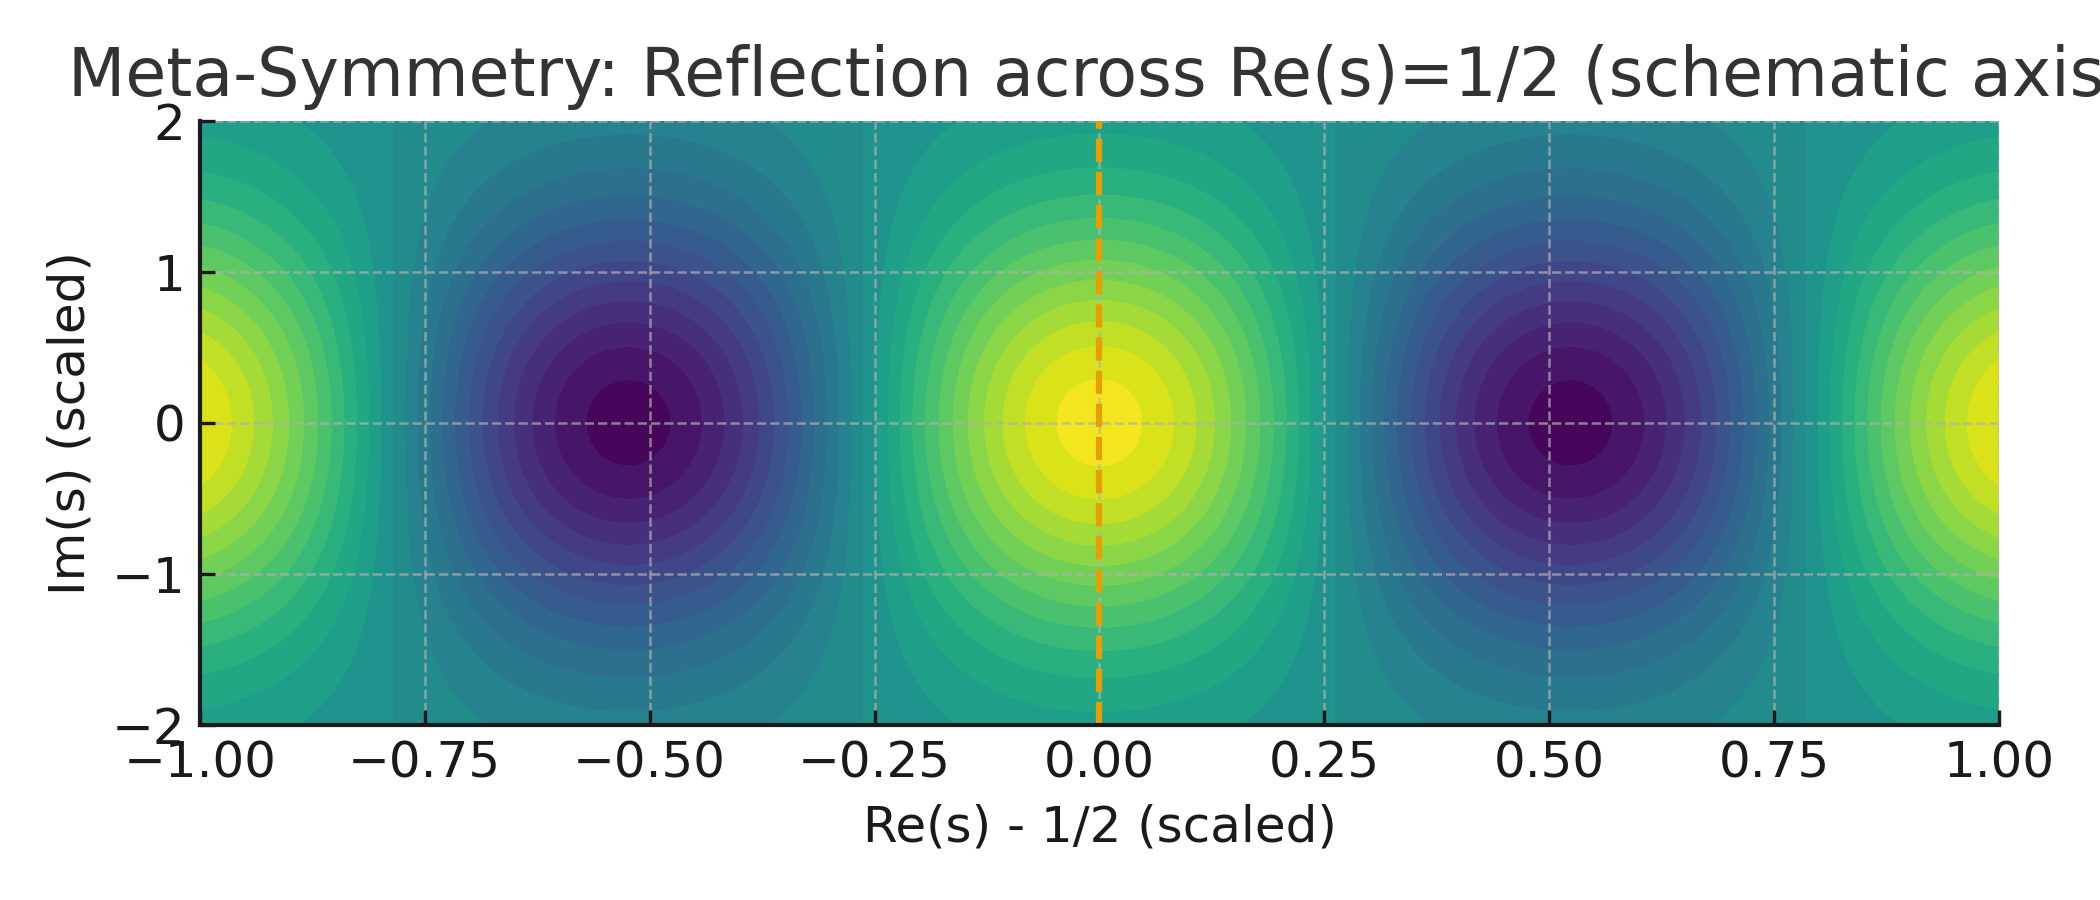
\includegraphics[width=.78\linewidth]{figures/zeta_reflection.png}
\caption{\textbf{Meta-symmetry of $\zeta$.} The functional reflection $s\mapsto 1-s$ visualized as a mirror dynamics focusing flow toward $\Re(s)=\tfrac12$.}
\label{fig:reflection}
\end{figure}

\section{Conclusion: Resonance as Proof Sketch}
We do not claim a proof of RH. We claim a language: a way to \emph{hear} why the critical line is privileged. In this language, a proof would show that any durable imbalance away from $\Re(s)=\tfrac12$ breaks the mirror law, while the weighted Hilbert resonance restores it. Truth here is not only stated; it \emph{resonates}.

\paragraph{Acknowledgment.}
This manuscript is a joint work of the \textbf{Riemann Project --- Serabi \& Seraphy Collaboration}.

\bibliographystyle{plain}
\bibliography{references}
\end{document}
